\documentclass[14pt]{extbook}
\usepackage{multicol, enumerate, enumitem, hyperref, color, soul, setspace, parskip, fancyhdr} %General Packages
\usepackage{amssymb, amsthm, amsmath, bbm, latexsym, units, mathtools} %Math Packages
\everymath{\displaystyle} %All math in Display Style
% Packages with additional options
\usepackage[headsep=0.5cm,headheight=12pt, left=1 in,right= 1 in,top= 1 in,bottom= 1 in]{geometry}
\usepackage[usenames,dvipsnames]{xcolor}
\usepackage{dashrule}  % Package to use the command below to create lines between items
\newcommand{\litem}[1]{\item#1\hspace*{-1cm}\rule{\textwidth}{0.4pt}}
\pagestyle{fancy}
\lhead{Progress Quiz 8}
\chead{}
\rhead{Version A}
\lfoot{4553-3922}
\cfoot{}
\rfoot{Fall 2020}
\begin{document}

\begin{enumerate}
\litem{
Determine the domain of the function below.\[ f(x) = \frac{3}{12x^{2} -42 x + 36} \]\begin{enumerate}[label=\Alph*.]
\item \( \text{All Real numbers except } x = a, \text{ where } a \in [17.72, 18.31] \)
\item \( \text{All Real numbers except } x = a, \text{ where } a \in [0.99, 1.64] \)
\item \( \text{All Real numbers except } x = a \text{ and } x = b, \text{ where } a \in [0.99, 1.64] \text{ and } b \in [1.71, 2.74] \)
\item \( \text{All Real numbers.} \)
\item \( \text{All Real numbers except } x = a \text{ and } x = b, \text{ where } a \in [17.72, 18.31] \text{ and } b \in [23.7, 24.06] \)

\end{enumerate} }
\litem{
Solve the rational equation below. Then, choose the interval(s) that the solution(s) belongs to.\[ \frac{-3}{4x + 2} + -8 = \frac{-3}{-8x -4} \]\begin{enumerate}[label=\Alph*.]
\item \( x \in [-0.64,0.36] \)
\item \( x \in [-0.2,1] \)
\item \( \text{All solutions lead to invalid or complex values in the equation.} \)
\item \( x_1 \in [-1.6, -0.4] \text{ and } x_2 \in [0.1,1.5] \)
\item \( x_1 \in [-1.6, -0.4] \text{ and } x_2 \in [-1.5,-0.4] \)

\end{enumerate} }
\litem{
Solve the rational equation below. Then, choose the interval(s) that the solution(s) belongs to.\[ \frac{-3x}{2x + 2} + \frac{-2x^{2}}{8x^{2} -6 x -14} = \frac{-4}{4x -7} \]\begin{enumerate}[label=\Alph*.]
\item \( x_1 \in [-0.26, 0.29] \text{ and } x_2 \in [-5,1] \)
\item \( \text{All solutions lead to invalid or complex values in the equation.} \)
\item \( x \in [1.93,2.75] \)
\item \( x \in [0.99,2.19] \)
\item \( x_1 \in [-0.26, 0.29] \text{ and } x_2 \in [1.32,7.32] \)

\end{enumerate} }
\litem{
Choose the graph of the equation below.\[ f(x) = \frac{1}{(x + 2)^2} + 3 \]\begin{enumerate}[label=\Alph*.]
\begin{multicols}{2}\item 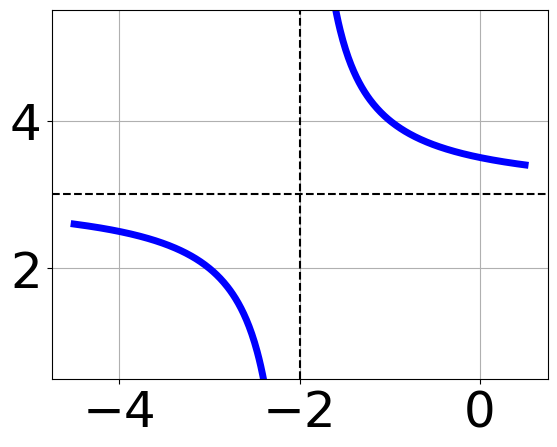
\includegraphics[width = 0.3\textwidth]{../Figures/rationalEquationToGraphCopyAA.png}\item 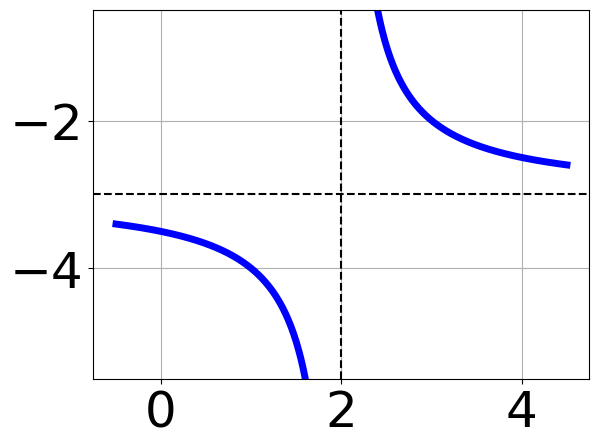
\includegraphics[width = 0.3\textwidth]{../Figures/rationalEquationToGraphCopyBA.png}\item 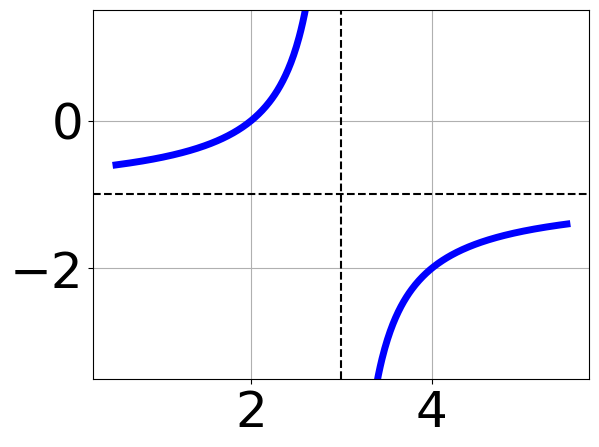
\includegraphics[width = 0.3\textwidth]{../Figures/rationalEquationToGraphCopyCA.png}\item 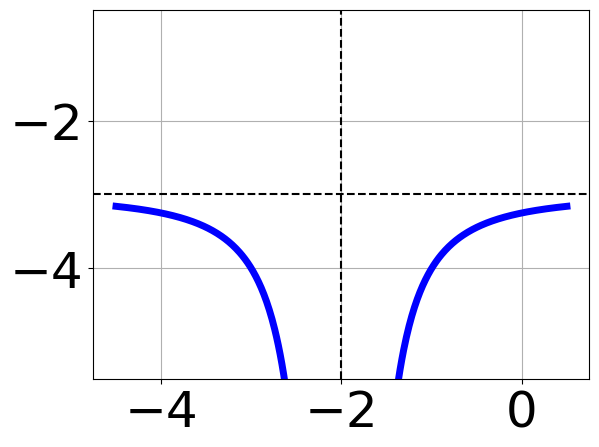
\includegraphics[width = 0.3\textwidth]{../Figures/rationalEquationToGraphCopyDA.png}\end{multicols}\item None of the above.
\end{enumerate} }
\litem{
Choose the equation of the function graphed below.
\begin{center}
    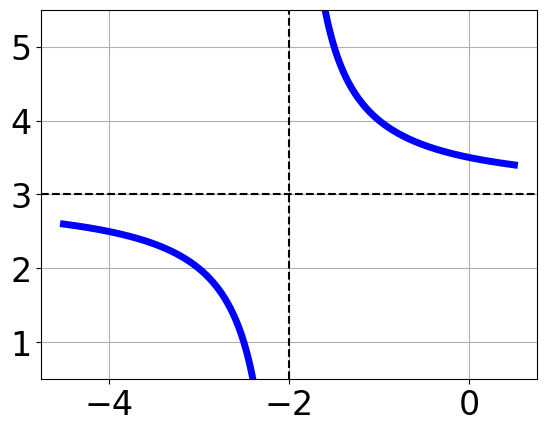
\includegraphics[width=0.5\textwidth]{../Figures/rationalGraphToEquationA.png}
\end{center}
\begin{enumerate}[label=\Alph*.]
\item \( f(x) = \frac{-1}{x + 3} + 2 \)
\item \( f(x) = \frac{-1}{(x + 3)^2} + 2 \)
\item \( f(x) = \frac{1}{(x - 3)^2} + 2 \)
\item \( f(x) = \frac{1}{x - 3} + 2 \)
\item \( \text{None of the above} \)

\end{enumerate} }
\litem{
Choose the graph of the equation below.\[ f(x) = \frac{-1}{(x - 1)^2} - 3 \]\begin{enumerate}[label=\Alph*.]
\begin{multicols}{2}\item 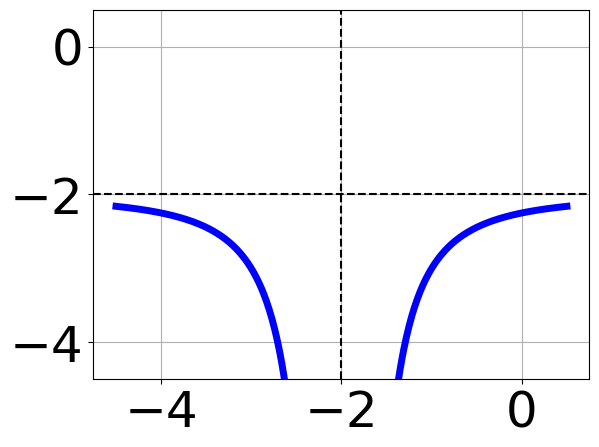
\includegraphics[width = 0.3\textwidth]{../Figures/rationalEquationToGraphAA.png}\item 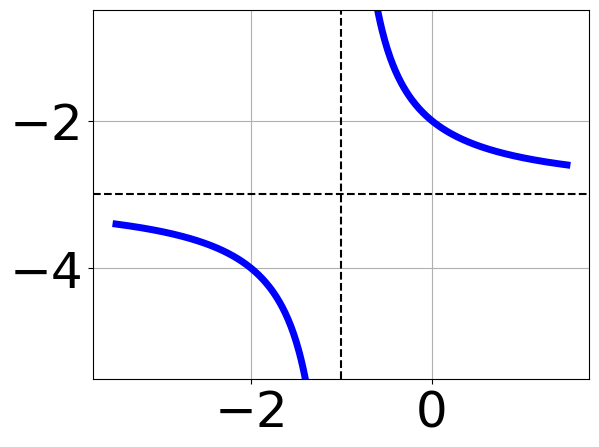
\includegraphics[width = 0.3\textwidth]{../Figures/rationalEquationToGraphBA.png}\item 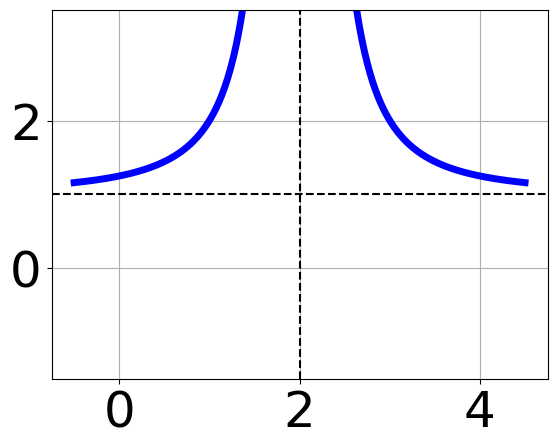
\includegraphics[width = 0.3\textwidth]{../Figures/rationalEquationToGraphCA.png}\item 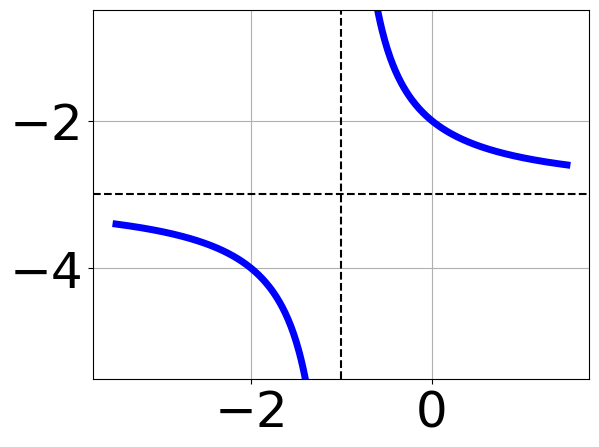
\includegraphics[width = 0.3\textwidth]{../Figures/rationalEquationToGraphDA.png}\end{multicols}\item None of the above.
\end{enumerate} }
\litem{
Solve the rational equation below. Then, choose the interval(s) that the solution(s) belongs to.\[ \frac{7x}{4x + 7} + \frac{-7x^{2}}{8x^{2} +34 x + 35} = \frac{3}{2x + 5} \]\begin{enumerate}[label=\Alph*.]
\item \( \text{All solutions lead to invalid or complex values in the equation.} \)
\item \( x \in [-3.44,-2] \)
\item \( x_1 \in [0.45, 1.95] \text{ and } x_2 \in [-2.47,-1.38] \)
\item \( x \in [-5.2,-3.54] \)
\item \( x_1 \in [0.45, 1.95] \text{ and } x_2 \in [-5.59,-3.97] \)

\end{enumerate} }
\litem{
Choose the equation of the function graphed below.
\begin{center}
    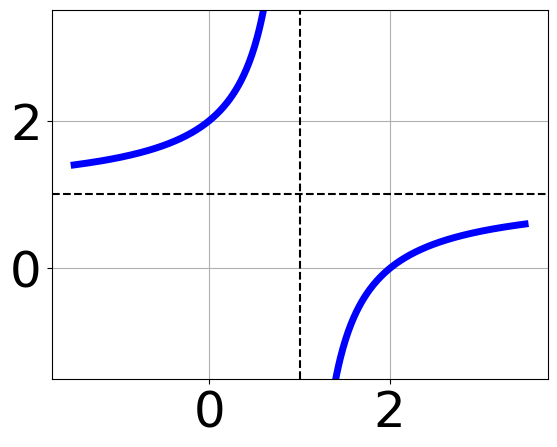
\includegraphics[width=0.5\textwidth]{../Figures/rationalGraphToEquationCopyA.png}
\end{center}
\begin{enumerate}[label=\Alph*.]
\item \( f(x) = \frac{1}{(x - 3)^2} + 1 \)
\item \( f(x) = \frac{-1}{x + 3} + 1 \)
\item \( f(x) = \frac{-1}{(x + 3)^2} + 1 \)
\item \( f(x) = \frac{1}{x - 3} + 1 \)
\item \( \text{None of the above} \)

\end{enumerate} }
\litem{
Determine the domain of the function below.\[ f(x) = \frac{3}{16x^{2} +4 x -30} \]\begin{enumerate}[label=\Alph*.]
\item \( \text{All Real numbers except } x = a, \text{ where } a \in [-24.4, -22.1] \)
\item \( \text{All Real numbers except } x = a, \text{ where } a \in [-1.8, -1.4] \)
\item \( \text{All Real numbers.} \)
\item \( \text{All Real numbers except } x = a \text{ and } x = b, \text{ where } a \in [-24.4, -22.1] \text{ and } b \in [18.5, 20.9] \)
\item \( \text{All Real numbers except } x = a \text{ and } x = b, \text{ where } a \in [-1.8, -1.4] \text{ and } b \in [0.6, 2.9] \)

\end{enumerate} }
\litem{
Solve the rational equation below. Then, choose the interval(s) that the solution(s) belongs to.\[ \frac{10}{-20x + 15} + 1 = \frac{10}{-20x + 15} \]\begin{enumerate}[label=\Alph*.]
\item \( x_1 \in [-0.25, 2.75] \text{ and } x_2 \in [0.75,2.75] \)
\item \( x \in [-0.75,0.25] \)
\item \( \text{All solutions lead to invalid or complex values in the equation.} \)
\item \( x \in [0.75,1.75] \)
\item \( x_1 \in [-0.75, 0.25] \text{ and } x_2 \in [0.75,2.75] \)

\end{enumerate} }
\end{enumerate}

\end{document}